\section{Description of Research Tasks, Progress, and Plans}
\label{sec:research}


\subsection{Progress and Accomplishments to Date}

The primary strategic objective of the NPNEQ CMS during the first 18 months of the funding period was to develop a \textbf{portable}, \textbf{extensible}, \textbf{scalable} and \textbf{reliable} DFT/RT-TDDFT framework that is fully compatible with existing petascale and near-term exascale~\cite{Kothe2019} \textbf{hybrid CPU-GPU} architectures.
We achieved this objective with the recent release of \textsc{inq}~\cite{Andrade2021}. 
In parallel, the team also pursued multi-institutional collaborative research efforts leading to science outcomes in the area of \emph{ultrafast materials science} using alternate tools and methodologies, some of which we will incorporate into the larger INQ ecosystem of codes in the future. 
Below is a summary of the software development and scientific research efforts within NPNEQ.

\subsubsection{Code Development}
\label{subsubsec:Code}
\paragraph{The INQ DFT/TDDFT platform}


With the widespread adoption of Graphical Processing Units (GPUs) as a powerful and energy efficient~\cite{Huang2009} hardware paradigm for scientific computing and the ongoing migration of DOE's national super-computing facilities from CPU to networked hybrid CPU-GPU architectures, it is of paramount importance within computational materials science that the community has access to electronic structure codes that are fully compatible with the emerging GPU computing landscape.
The INQ platform~\cite{Andrade2021} under development by the NPNEQ team addresses this need within the context of Density Functional Theory (DFT)-based approaches to materials simulation while further specializing to non-perturbative simulations of materials under non-equilibrum conditions.
During the first 18 months of this funding period, the NPNEQ center accomplished the design and development tasks necessary to deliver a modular and extensible GPU-accelerated software solution for DFT/TDDFT led by LLNL PIs \textbf{Andrade} and \textbf{Correa}.
Below we outline the unique design features of INQ as well as its current capabilities.

\noindent{\bf General features and design:} The design philosophy of INQ differs in many important respects from established Fortran/C-based DFT/TDDFT codes developed in past decades to run on CPUs: Unlike the CPU computing model that matured decades ago, GPU computing is still rapidly evolving with different hardware designs competing for primacy in the super-computing space and vendors making significant low-level updates and optimizations on a regular basis.
\textsc{Inq} is designed from the outset to be easily modified and improved on top of evolving hardware, while providing consistent results and behavior independent of specific vendor platforms. 
\textsc{Inq} achieves this goal through abstractions enabled by modern C++ programming, by implementing a clear separation between different classes of software components, namely: application (DFT/TDDFT) specific code, infrastructure (basis-set, boundary conditions, data-structures, etc.) code and low-level numerical library (blas, FFTs, etc.) code. 
\newline 
\newline
As shown in Figure~\ref{fig:inq_design}(a), in traditional DFT/TDDFT programs, the different software components are rather tightly coupled into monolithic software units, and the programmer may encounter all classes of code within a given subroutine or function. 
\textsc{Inq} in contrast implements a hierarchical structure with an application (DFT/TDDFT) code layer that sits on top of an infrastructure library layer that handles all hardware-dependent decisions. 
A programmer working with the DFT/TDDFT layer then encounters a much simplified programming interface that syntactically resembles the relevant physics equations~(see Ref.~\cite{Andrade2021}) and is shielded from lower-level representation-specific and hardware-specific details. 
This hierarchical design is critical for developing code that is hardware portable while simultaneously reducing the learning curve for new developers from the DFT community to be able to quickly add functionality in the application layer. 
Note that while interpreted scripting languages such as Python, MATLAB, etc. can provide a similar type of abstraction, there is an associated performance cost that is not incurred by \textsc{inq} as it relies on compiled C++.

\begin{figure}[h]
	\centering
	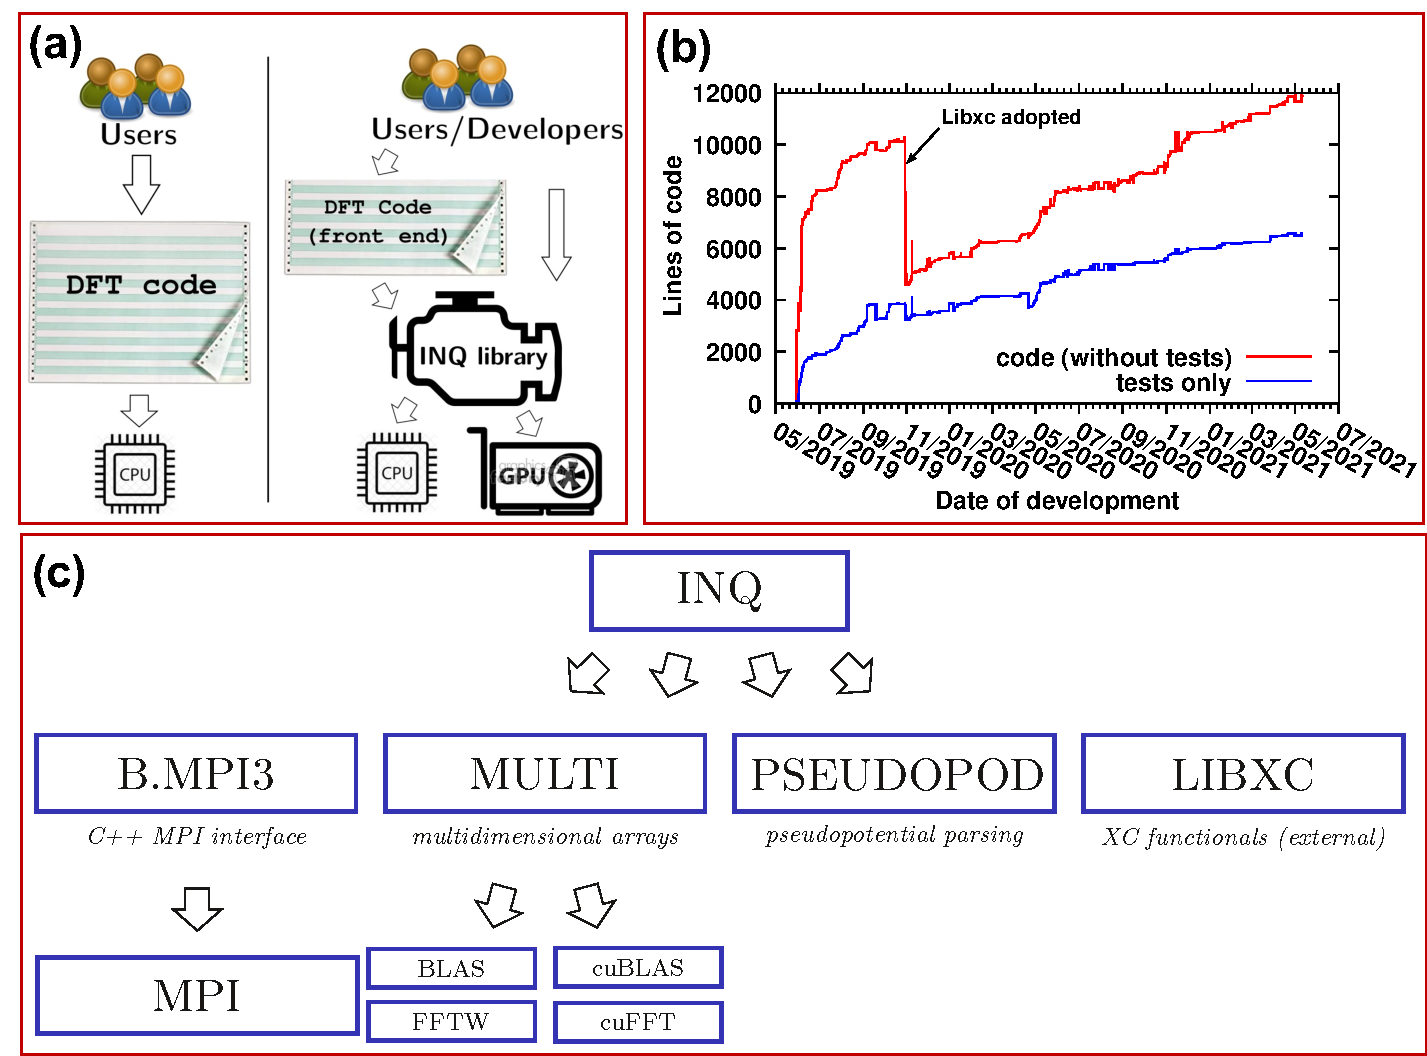
\includegraphics[width=0.8\linewidth]{figures/INQ_design_features.pdf}
	\caption{%\small
		Key design features of the INQ framework.
		(a) INQ was built from the outset as a library that can operate on both CPU and GPU hardware.
		(b) At roughly 12,000 lines of code, INQ is extremely lightweight compared to other DFT/TDDFT codes offering comparable functionality.
		Adopting GPU-compatible \textsc{libxc} substantially reduced the size of INQ's internal codebase.
		(c) INQ brings together a highly modular hierarchy of libraries ensuring maximum adaptability with respect to future hardware and software changes.
	}
	\label{fig:inq_design}
\end{figure}

The hardware portability of \textsc{inq} is achieved through a highly modular design of its library layer which brings together a number of different components that were developed at LLNL and the extended DFT community. 

Some of the key libraries used in INQ are:
\begin{itemize}
	\item \textbf{MULTI:} Developed by PI \textbf{Correa} at LLNL, \textsc{MULTI} provides multidimensional array access on both CPU and GPU memory models while abstracting operations over arrays without compromising maximum performance. 
	It also provides the interface between \textsc{inq} and vendor-provided linear algebra, FFT and C++ standard libraries.
	\item \textbf{B.MPI3:} B-MPI3 is a C++ library wrapper for version 3.1 of the Message Passing Interface (MPI) standard that simplifies its utilization while maintaining a similar level of performance as the more cumbersome native MPI C-language interface. 
	B.MPI3 was developed by PI \textbf{Correa} at LLNL.
	\item \textbf{PSEUDOPOD:} \textsc{PSEUDOPOD} is a CPU+GPU compatible library that handles pseudopotential (PP) parsing, filtering, and other auxiliary tasks while supporting many popular PP formats as well as standardized PP sets such as Pseudodojo~\cite{Van2018} and SG15~\cite{Schlipf2015}. 
	\textsc{PSEUDOPOD} developed by PI \textbf{Andrade} at LLNL, moves PP handling from the application layer to the library layer of INQ.
	\item \textbf{LIBXC:} Libxc is a standalone library of exchange and correlation (XC) functionals initially developed by M. Marques~\cite{Marques2012}. 
	As part of the development on \textsc{inq}, PI \textbf{Andrade} implemented a GPU extension of \textsc{libxc} that relies on cuda ‘unified memory’ to store its internal data structures. 
	\textsc{INQ} therefore has the ability to evaluate XC functionals on GPUs, which is critical to maintain all data in the GPU.
\end{itemize}

Figure~\ref{fig:inq_design}(c) shows the interaction between these \textsc{inq} modules and lower-level vendor-provided libraries. 
The modularization of \textsc{inq}'s library layer affords several advantages; e.g., different components can be developed and tested independently as well as shared with other codes, to avoid duplication of work and enable collaborative development. 
Following changes to low-level hardware-optimized libraries, only a small portion of the code needs to be updated in a way that is transparent to application layer developers. 
Furthermore, by creating libraries and offloading tasks to them whenever possible, the codebase internal to \textsc{inq} can be kept relatively small as shown in Fig.~\ref{fig:inq_design}(b). 

Finally, in order to ensure reliability within a collaborative environment, \textsc{inq} adopts a test-driven development (TDD)~\cite{Beck2002} approach in line with modern software development best practices. 
Therefore, the \textsc{inq} codebase consists of both unit and functional tests that are run regularly within an automated continuous delivery platform hosted on gitlab. This workflow ensures that only code modifications that do not lead to errors anywhere in the codebase are accepted.

The result is a fully functional yet lightweight DFT/TDDFT framework that is portable across hardware platforms and offers optimal scaling on distributed hybrid CPU-GPU platforms combined with reliable numerical accuracy. 
\textsc{Inq}'s DFT/TDDFT application layer currently implements semi-local DFT total energies, forces, and real-time propagation of the time-dependent KS equations within the adiabatic XC approximations for both molecular and solid-state systems within a periodic supercell framework. 
Below we discuss performance and validation tests of these capabilities within \textsc{inq}. 

\noindent{\bf GPU-MPI functionality and scaling:} \textsc{Inq} is the first implementation of DFT and DFT TDDFT that is written \emph{from scratch} to work on GPUs.
It has proven quite challenging to adapt an existing code to run on the GPU, as extensive modifications to the whole code are needed.
For this reason, we started a new code, designed from the ground up, that runs on GPUs and CPUs. 

We studied available platforms for high-level GPU programming such as \textsc{raja}~\cite{Beckingsale2019}, \textsc{Kokkos}~\cite{CarterEdwards2014}, \textsc{OpenMP}~\cite{Lee2010} and \textsc{SyCL}~\cite{Alpay2020} but could not find one that was directly suitable for the operations needed for DFT/TDDFT and that was mature enough when we started the project (mid-2019).
Therefore, we designed our code using the \textsc{cuda} C++ extensions with a thin layer of abstraction on top, which allows us to make most of the code independent of the GPU backend.

\textsc{Inq} achieves distributed memory parallelism (parallelism between several nodes) by using the Message Passing Interface (\textsc{MPI}) infrastructure.
For simplicity, it uses one MPI task per GPU, e.g., in LLNL's Lassen, each of the 4 GPUs in a node is controlled by 1 MPI task.

In \textsc{inq} we directly call \textsc{MPI} over data in GPU memory.
Ideally, most modern \textsc{MPI} implementations are GPU-aware and can recognize the GPU memory space, and they can directly access data.
In the best scenario, they can also communicate the data to and from GPU memory without passing through main memory, but this is not always the case.
For non-GPU-aware implementations, \emph{managed memory} residing on the GPU would be automatically copied to main memory before \textsc{MPI} calls.
Unfortunately, this last case has a non-negligible overhead in the communication cost.

\begin{figure}[h]
	\centering
	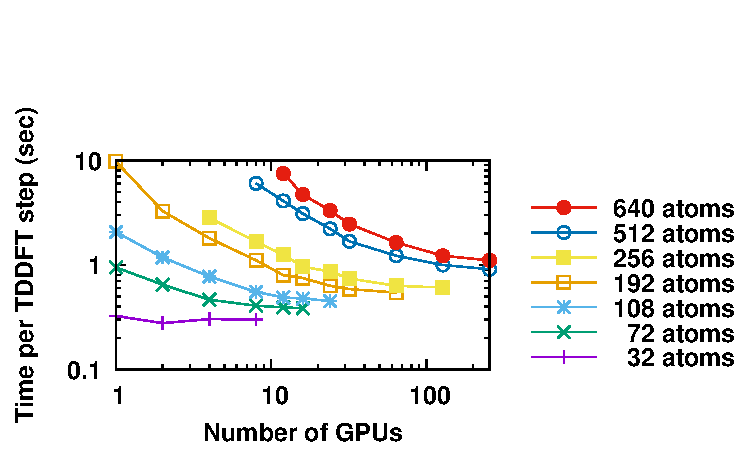
\includegraphics[width=0.5\linewidth]{figures/scaling/strong}
	\caption{\small
		Strong scaling plot: wall time per TDDFT simulation step for Aluminum FCC supercell.
		These simulations are run in LLNL's Lassen supercomputer (NVIDIA Volta 100 GPU).
	}
	\label{fig:scaling_strong}
\end{figure}

\begin{figure}[h]
	\centering
	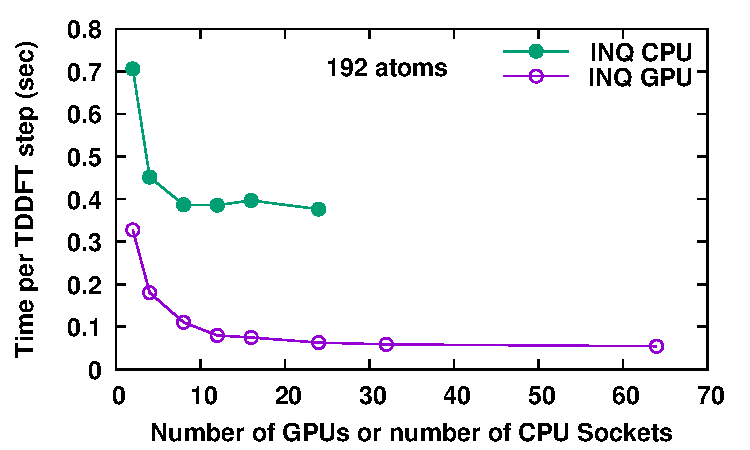
\includegraphics[width=0.45\linewidth]{figures/scaling/gpu_vs_cpu}
	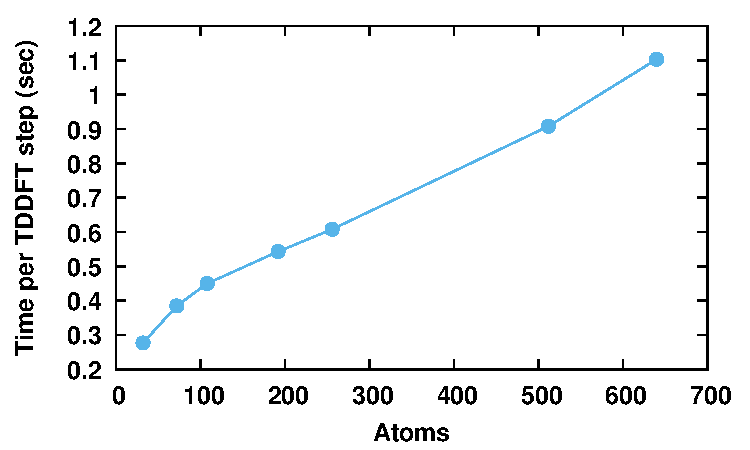
\includegraphics[width=0.45\linewidth]{figures/scaling/weak}
	\caption{\small
		(left)  Comparison of INQ GPU and CPU implementations TDDFT timings for Aluminum FCC supercell.
		(right) Best timing achieved for variable system size (\emph{Weak} scaling).
		These simulations are run in LLNL's Lassen supercomputer (NVIDIA Volta 100 GPU).
	}
	\label{fig:scaling_gpu_vs_cpu}
	\label{fig:scaling_weak}
\end{figure}

The main limitation to scalability is the lack of a parallel FFT library for GPUs~\cite{Ayala2020}. 
Our own basic implementation doesn't scale very well; i.e., our parallelization only covers one degree of freedom (the states) and not the space (domains), which is why we see the time per iteration in the weak scaling going up in Figure~\ref{fig:scaling_weak}.
Despite the incomplete parallelization, iterator times are below a second per step, even with a few hundred atoms, which is very competitive among alternative codes.
Excellent strong scaling of INQ code on GPUs  is clearly seen in Figure~\ref{fig:scaling_strong}. 
\begin{figure}[h]
	\centering
	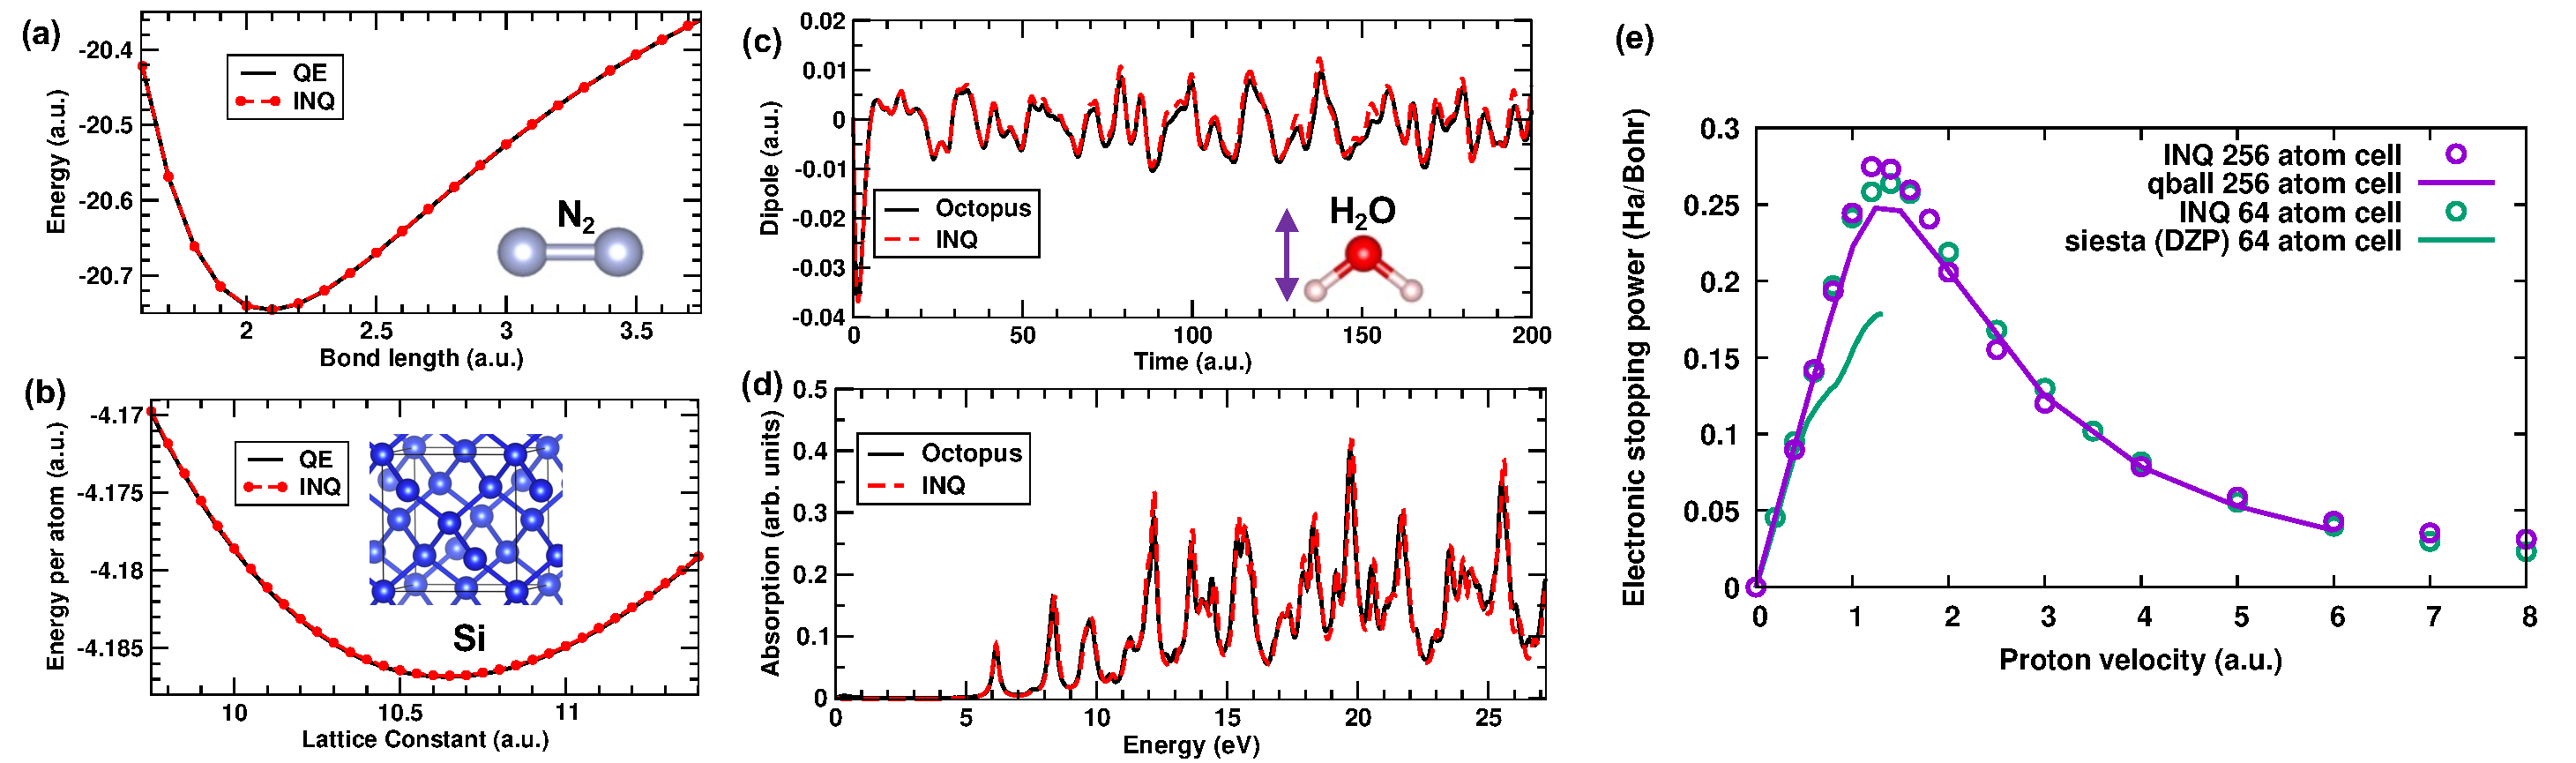
\includegraphics[width=1.0\linewidth]{figures/Results-Fig.pdf}
	\caption{%\small
		(Adapted from Ref.~\cite{Andrade2021}.) 
		Comparison between \textsc{inq} and the established electronic structure codes \textsc{Quantum Espresso} (QE) and \textsc{octopus}.
Results for ground state total energies and real-time TDDFT optical response are shown. 
		(a) Total energy vs bond length in \(\mathrm{N_2}\).
		(b) Total energy vs lattice constant in bulk silicon. 
		(c) Time evolution of the dipole moment in gas phase \(\mathrm{H_2O}\) following a ``kick'' perturbation. 
		(d) Linear optical absorption of molecular \(H_2O\). 
		In all cases, there is a high level of agreement between the codes.
		(e) Electronic stopping power obtained by direct simulation of a proton projectile moving in aluminum atom fcc supercell with different codes: \textsc{inq}, \textsc{qball} (from Ref.~\cite{Schleife2015}) and \textsc{siesta} with atom-centered double-zeta plus polarization basis (DZP) (from Ref.~\cite{Correa2012}).
		Each point is obtained by evaluating the steady energy rate dissipation.
		All simulations are with 3 valence (explicitly simulated) electrons per aluminum which is enough for channeling stopping power.
	}
	\label{fig:inq_results}
\end{figure}
\newline
\noindent{\bf Validation of results:} For a new scientific code, it is fundamental to produce results that are consistent with other approaches and codes. 
As \textsc{inq} follows a test-driven development approach, \textsc{inq}'s codebase is continuously tested and validated at multiple levels against analytical results or benchmark data obtained from other established codes such as \textsc{Quantum Espresso}~\cite{Giannozzi2009}. 
We recently carried out higher-level end-to-end tests of \textsc{inq} as a part of the software release validating \textsc{inq} results against corresponding quantities obtained from established plane-wave and realspace grid codes: \textsc{Quantum Espresso} (QE) and \textsc{Octopus}~\cite{Tancogne2020}. 
For this purpose, we chose observables such as molecular bond lengths and crystal lattice parameters based on total-energy minimization, as well as linear optical response from real-time propagation as the relevant quantities to be compared. 
For details on calculation parameters, please refer to Ref.~\cite{Andrade2021}. 
As is apparent from the comparisons shown in Figure~\ref{fig:inq_results}, absolute total energies from \textsc{inq} are within \(0.3~\mathrm{mHartree/atom}\) of the QE reference. 
Furthermore, the optical response of a gas phase water molecule as obtained from \textsc{inq} is in excellent agreement with the corresponding result from \textsc{octopus} in the time domain (Figure~\ref{fig:inq_results}(c)) and therefore excitation frequencies in the optical absorption spectrum are also found to match closely across a wide energy range. 

% \begin{figure}
% 	\centering
% 	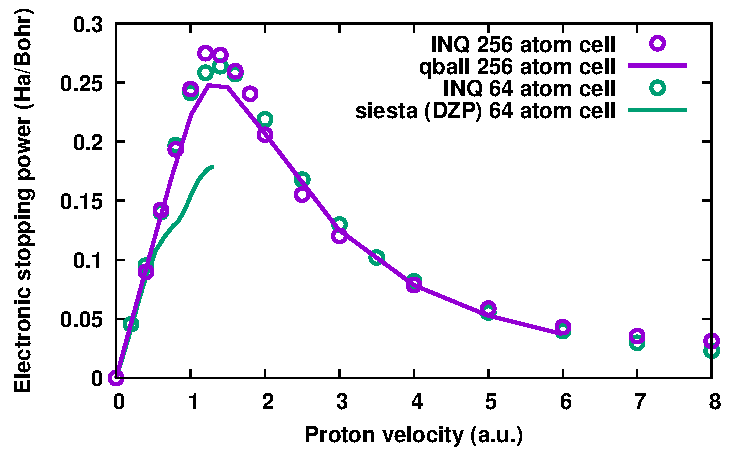
\includegraphics[width=0.66\columnwidth]{figures/al_stopping}
% 	\caption{
% 		Electronic stopping power obtained by direct simulation of a proton projectile moving in aluminum atom fcc super cell with different codes: \textsc{inq}, \textsc{qball} (from Ref.~\cite{Schleife2015}) and \textsc{siesta} with atom-centered double-zeta plus polarization basis (DZP) (from Ref.~\cite{Correa2012}).
% 		Each point is obtained by evaluating the steady energy rate dissipation.
% 		All simulations are with 3 valence (explicitly simulated) electrons per aluminum which is enough for channeling stopping power.
% 	}
% 	\label{fig:al_stopping}
% \end{figure}

Finally, \textsc{inq} was tested against a medium-to-high energy application, namely electronic stopping power (Figure~\ref{fig:inq_results}(e)). 
Despite the association with other areas of research, such as fusion and radiation damage, electronic stopping power plays an important role in the development of the theory of solids~\cite{Thomson1912, Darwin1912, Bohr1913} and the electron gas~\cite{Lindhard1964}.
Furthermore, by interpreting the electron-phonon coupling as low velocity limit of stopping power, TDDFT offers the only scalable method to non-perturbative access to calculate electron-phonon coupling in complicated systems or at finite temperature~\cite{Caro2015}. 
To develop this method, it is important to achieve reliable electronic stopping power in the regime of a tenth to a hundredth of atomic unit of velocity, in a variety of atomistic environments. 
This is the topic in the NPNEQ's publication Ref.~\cite{Quashie2020} where a record low value of ion velocity \(0.04~\mathrm{a.u.}\) is achieved in a non-adiabatic calculation and its relation with the electronic density of state at the Fermi level is established.

\paragraph{Tight binding model for non-equilibrium dynamics}\label{sec:tight-binding}

Within NPNEQ, \emph{ab initio} code development efforts led by LLNL and SLAC teams are complemented by efforts at LBNL to develop tight-binding models for non-equilibrium dynamics with the recognition that feedback between qualitative models and quantitative simulations is broadly beneficial for knowledge generation within materials science. 
In particular, careful model building based on first-principles calculations combined with large-scale model simulations is a promising route to produce interesting insights into the dynamic behavior of  materials driven far from equilibrium. 
We have developed an atomic-orbital-based tight-binding code for simulations on large time and length scales to supplement the capabilities of \textsc{inq}. 
These models treat charge, spin, orbital, and atomic degrees of freedom explicitly, capturing the quantum effects of charge carriers, the non-collinear spin dynamics, and the cooperative lattice vibrations. 

With the current tight-binding code, structural and electronic optimization can be performed to study ground state properties. 
For simulating relaxation dynamics of excited solids, the code supports Ehrenfest dynamics and Car-Parrinello dynamics. 
The effect of linearly polarized light field is implemented via the Peierls substitution method. 
Our recently published work on manganites~\cite{Rajpurohit2021} demonstrates the potential of such tight-binding models to study non-equilibrium dynamics in functional quantum materials. 

During the project period, we extended the code to simulate multilayer oxide structures, layered transition metal dichalcogenides (TMDC), and circularly polarized excitations. 
This has led to multiple scientific outputs and insights both through intra-NPNEQ~\cite{Rajpurohit2021} and external collaborations~\cite{Siddiqui2020} as outlined in the next subsection. 
Work is in progress to implement further extensions such as spin-orbit couplings, van der Waals (vdW) interactions, and Nose-Hover thermostat to incorporate finite-temperature effects. 
Additionally, the inclusion of external magnetic fields will allow for the simulation of magnetic excitations and magnon dispersion. 
Solving for these spin-waves will be done in large unit cells using an effective spin Hamiltonian consisting of Zeeman effects, exchange interactions, and magnetic
anisotropies. 

\subsubsection{Collaborative Science}
\label{sec:collaborative}

\paragraph{Role of non-equilibrium spin-phonon coupling in enhancing bulk photovoltaic effect}\label{sec:BPVE}

During the project period, our work on the materials system of \(\mathrm{Pr_xCa_{1-x}MnO_3}\) has resulted in the discovery of a new way to enhance the bulk photovoltaic effect by optically induced phase transitions. 
These results, currently under review, are reported in the preprint Ref.~\cite{Rajpurohit2021}. 
Our study provides a unified picture of the photocurrent generation and its evolution through real-time simulations, and will have a significant impact in field of the bulk photovoltaic effect (BPVE) where understanding, predicting, and ultimately controlling the photovoltaic behavior remains a challenge.
We show theoretically that this strongly correlated oxide perovskite displays strong photocurrent enhancement when it is driven into a hidden magnetic phase transition (See Figure~\ref{fig:PCMO}).
This phenomenon is highly non-perturbative, and lies outside the perturbative paradigm of shift and ballistic currents used in this field. 
The maximum photoresponsivity obtained is almost an order of magnitude higher than that reported for other transition metal oxides such as \(\mathrm{BiFeO_3}\) and \(\mathrm{BaTiO_3}\).

\begin{figure}[ht]
	\centering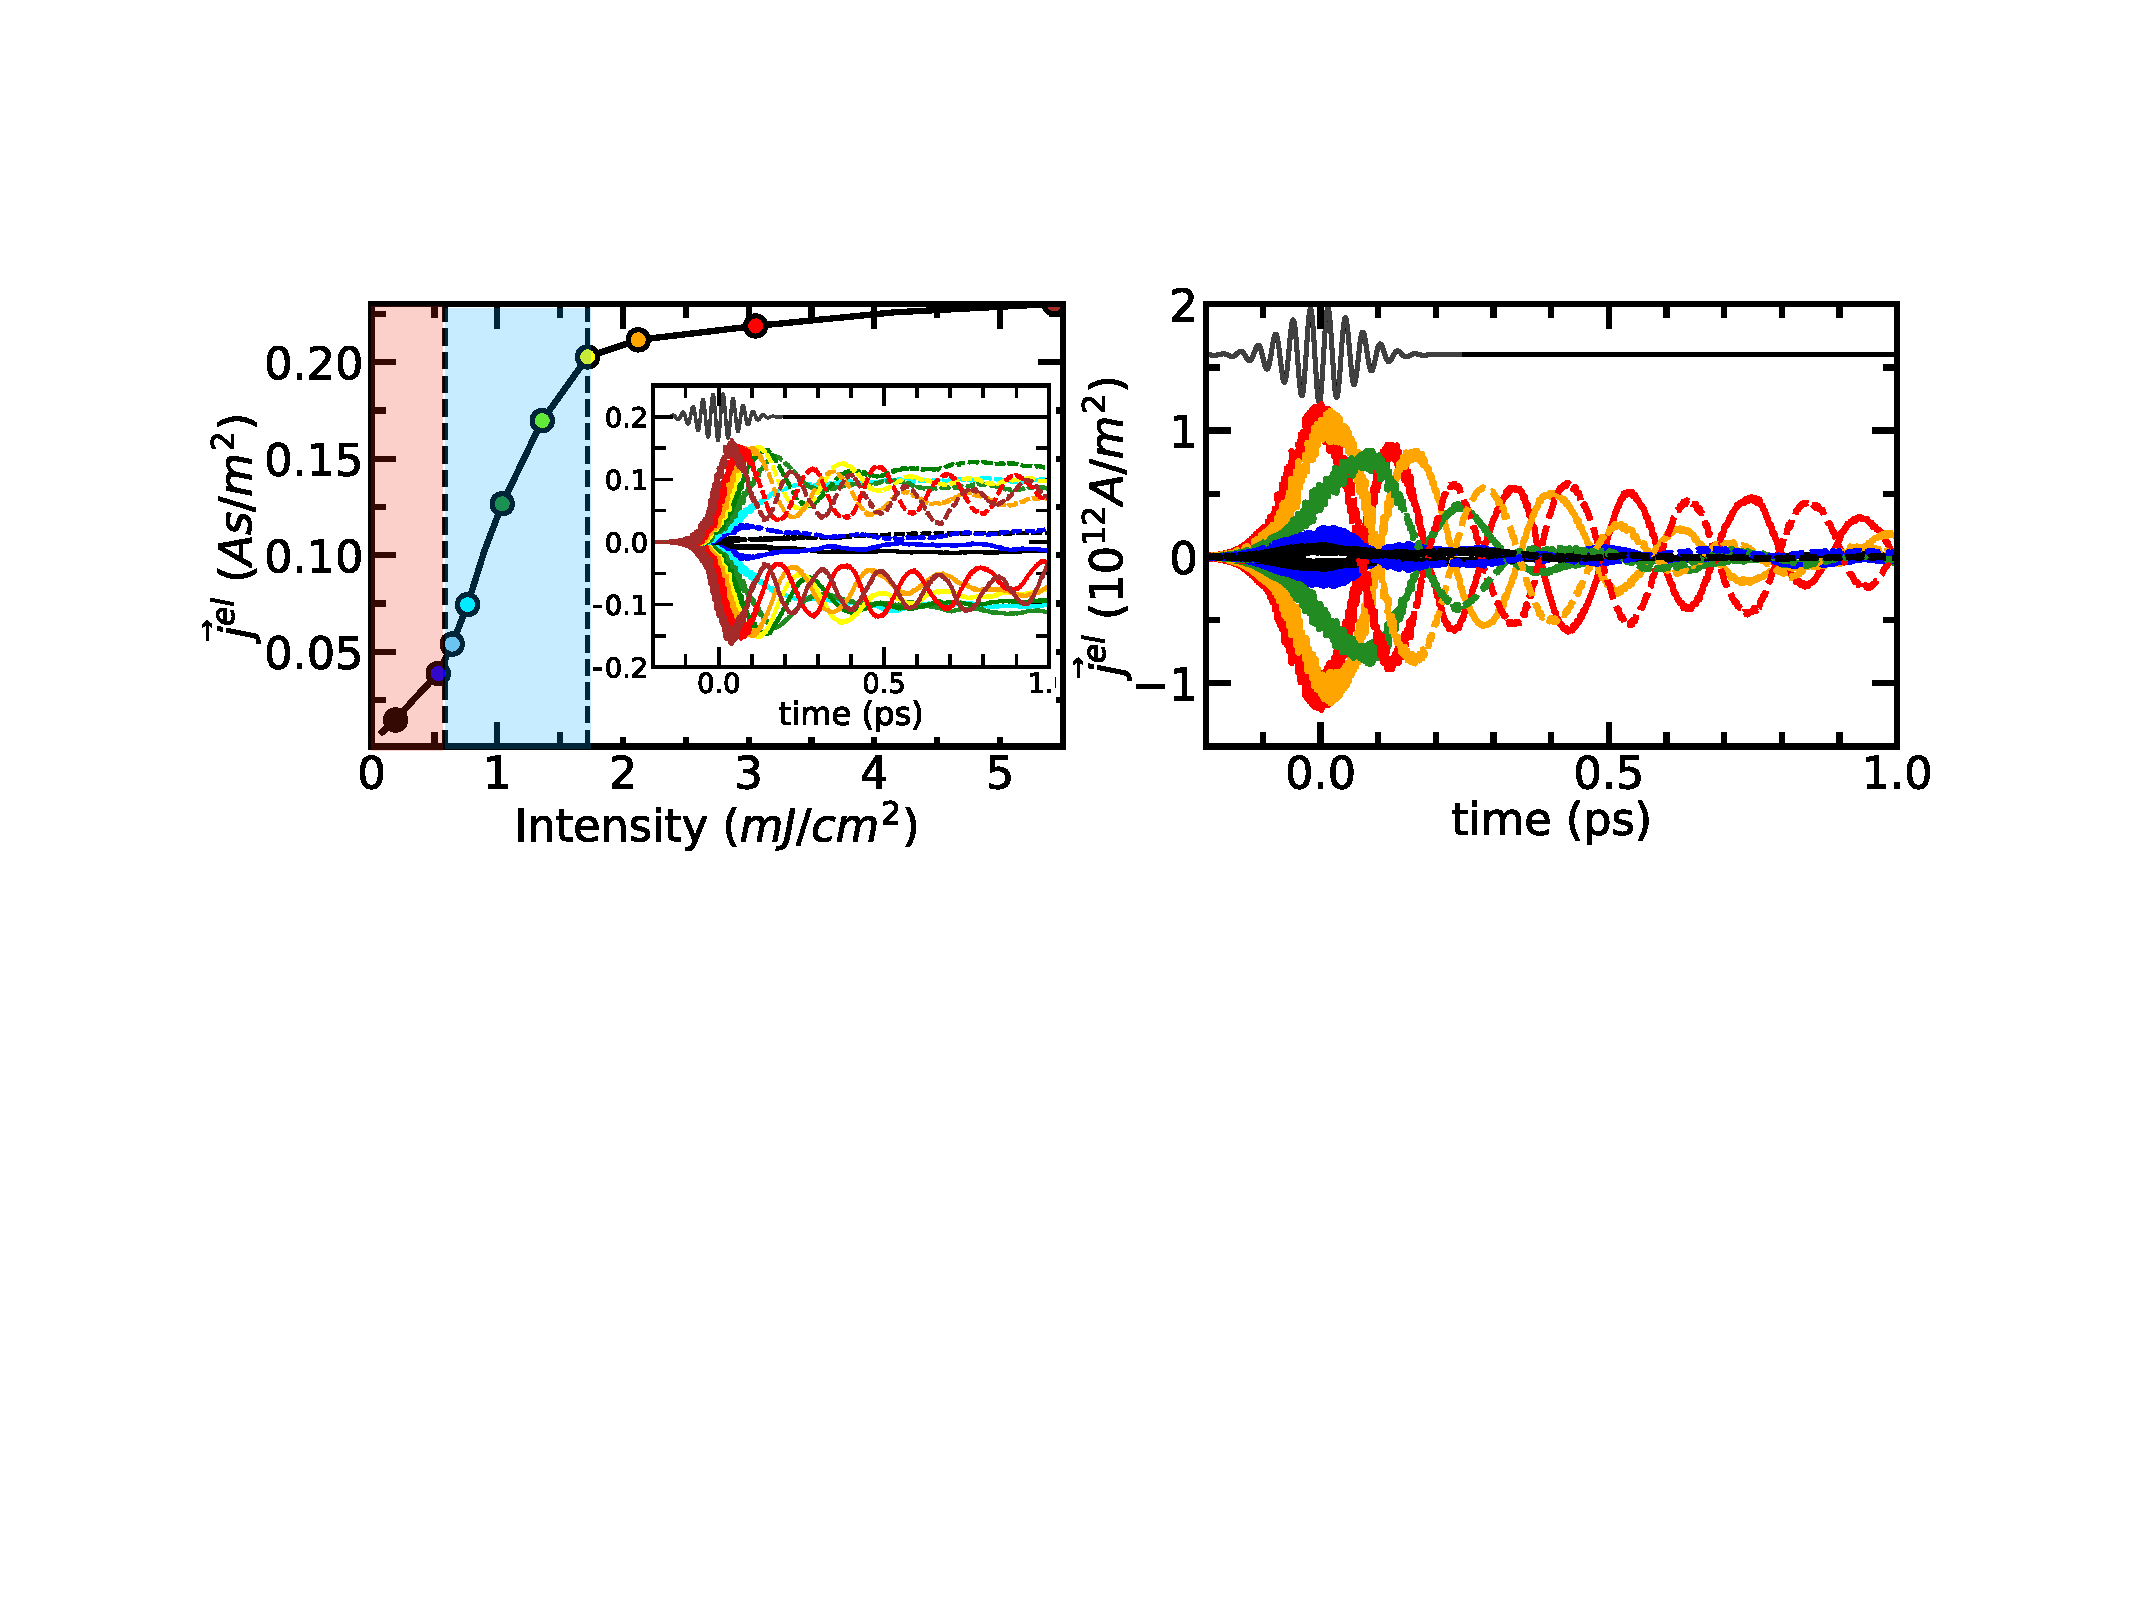
\includegraphics[width=0.8\linewidth]{figures/photocurrent_old}
	\caption{%\small
		Simulated photocurrent of \(\mathrm{Pr_xCa_{1-x}MnO_3}\), as a function of light intensity and time after excitation. 
		Rapid enhancement of photocurrent (left) is indicative of a non-perturbative process beyond the frameworks of previously studied shift and ballistic current theories.
	}
	\label{fig:PCMO}
\end{figure}

To study this effect, we use a methodology based on real-time simulations of a first-principles-based Hubbard model which treats all the relevant degrees of freedom, namely charge, spin, orbital, and lattice, explicitly. 
Our methodology allows us to study transient effects such as THz oscillations and their decay on picosecond timescales, as well as current saturation at higher light intensities, all of which are inaccessible using perturbative frequency domain techniques that have been in use for BPVE. 

In this work, {\bf Tan} has supervised photocurrent simulations, {\bf Pemmaraju} has provided input on the handling of dissipative processes, and {\bf Ogitsu} has guided the research focus to questions that can be answered in greater detail using the \textsc{inq} code in the remaining project period. 
Follow-up work will utilize the exact-exchange functional features of the \textsc{inq} code to explore the impact of non-local exchange on photocurrents in these strongly correlated systems. 
We will use GPU optimization of the \textsc{inq} code to extend these simulations to the relevant time scales identified above.  

\paragraph{Effect of surface defects on carrier dynamics in lead halide perovskites}

High defect tolerance has been considered as a main reason for the long charge carrier lifetime and high photoluminescence quantum yield in bulk lead halide perovskites (LHPs). 
On the other hand, surface defects play a critical role in determining charge carrier dynamics and optical properties, especially for LHP nanocrystals and quantum dots. Therefore, revealing the nature of surface defects and developing a strategy for their effective passivation are of strong interest. 
{\bf Tan} and {\bf Ogitsu}, together with collaborators at UCSC~\cite{Smart2021}, have used first-principles calculations to reveal that interstitial and antisite defects in a prototypical LHP, \(\mathrm{CsPbBr_3}\), can have lower formation energy when they form at the surface instead of bulk while simultaneously creating deep trap states within the bandgap.
We show how to choose molecular ligands to passivate these defects, eliminating trap states in favor of shallow states, which enhances photoluminescence 
(See Figure~\ref{fig:defect}). This work has implications for  the field of LHPs, especially LHP devices where interfacial chemistry plays an important role in the optoelectronic properties and stability.

This work forms the basis for planned real-time simulations of lossy processes at these defects in the LHPs, such as non-radiative recombination processes and dephasing, which are of fundamental interest for optoelectronic applications. 
Even though typical RT-TDDFT simulations are shorter than the natural time scales of these processes, it has been demonstrated that their rates can still be extracted, by using a cumulant expansion approach~\cite{Qiao2020}. 
Scalability of the \textsc{inq} code will enable these calculations in challenging systems such as LHP surfaces defects, which contain a large number of electrons.     

\begin{figure}[h]
	\centering
	\begin{minipage}[b]{.48\textwidth}
		\centering
		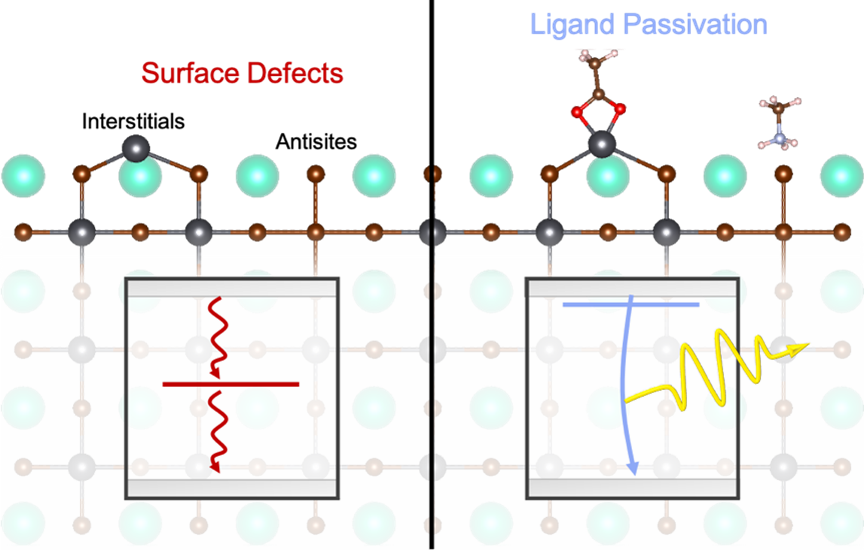
\includegraphics[width=0.99\textwidth]{figures/defect_passivation} 
		\caption{%\small
			Schematic atomic structure of defects at the surface of \(\mathrm{CsPbBr_3}\), which are susceptible to non-radiative recombination when unpassivated (left), but become less detrimental to radiative recombination when passivated (right).
			\label{fig:defect}
		}
	\end{minipage}
	~
	\begin{minipage}[b]{.48\textwidth}
		\centering
		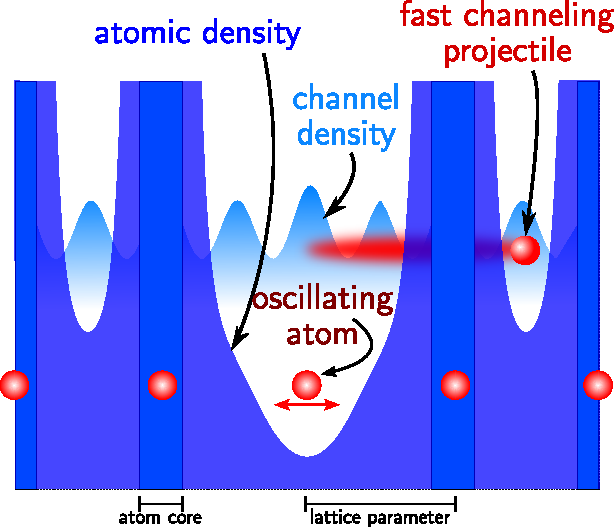
\includegraphics[width=0.8\textwidth]{figures/stopping_eph}    \\
		\caption{%\small
			Schematic image describing relation between stopping power and el-ph. Stopping power: coupling between projectile and electrons. El-ph: coupling between oscillating atoms and electrons. See page \pageref{page:stopping_eph}. 
			\label{fig:stopping_eph}
		}
	\end{minipage}
\end{figure}

% \begin{figure}
% \centering

% \caption{
% 	Electron-phonon coupling seen as an electronic-stopping power process. 
% 	The analogy is that, while a fast intruding projectile is stopped by the host electrons (channel or off-channel densities), an oscillating atom from the host is subject to the friction of the electrons present around the atomic site.
% }
% \label{fig:stopping_eph}
% \end{figure}
% \textcolor{red}{Descriptions of selected type-B projects.}

\paragraph{Ultrafast dynamics in strong-field ionized liquid water} 

% \begin{figure}[h]
% 	\centering
% 	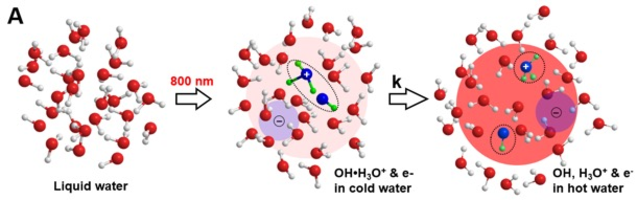
\includegraphics{figures/Water}
% 	\caption{
% 		The ionization of liquid water and formation of solvated \(\mathrm{H_3O^+}\), \(\mathrm{OH\cdot}\) radical and electron species is followed by the local thermalization involving energy exchange between the electronic and ionic degrees of freedom.
% 	}
% 	\label{fig:water}
% \end{figure}

Photo-excitation-induced structural dynamics in liquid water represents a paradigmatic case of excited state electron-ion dynamics in the condensed phase. 
In particular, the radiolysis of liquid water and its aftermath is a process of fundamental importance in a variety of technological contexts~\cite{Garrett2005} such as energy harvesting, biochemistry, biomedicine, corrosion mitigation, etc. 
Therefore, investigating the interplay between the electronic and ionic degrees of freedom in photo-ionized liquid water on the femto-picosecond timescales relevant to the creation and transformation of short-lived reaction intermediates~\cite{Loh2020} is of interest to both experiment and theory.
Within the current funding period, NPNEQ researchers at SLAC collaborated with experimental teams working at SLAC's MeV-UED instrument to uncover the structural fingerprints of hydronium cation-hydroxyl radical pairs on femtosecond timescales in strong-field ionized liquid water. 
In this study, we deployed velocity-gauge real-time TDDFT as implemented within the \textsc{salmon} code~\cite{salmon} to estimate the photo-ionization fraction in liquid water for experimentally relevant laser pulse parameters. 
Our simulations revealed a non-linear multi-step photo-ionization process in liquid water subjected to high-intensity near-infrared radiation, and our predicted excited electron energy distribution subsequently informed classical models of thermalization based on molecular dynamics. 
A manuscript summarizing the findings of our experiment-theory collaboration is currently under review in \emph{Science}.
In the near future, we plan to further extend our studies in this prototypical water system by simulating non-adiabatic Ehrenfest electron-ion dynamics during and after laser illumination using our RT-TDDFT platform \textsc{inq} and comparing our results with recent ultrafast experiments. 

%\subsubsection{WTe2 collaborations}

\paragraph{Charge density wave melting in 2D materials}

In this experimental collaboration~\cite{Siddiqui2020}, we perform the first ultrafast investigation of \(\mathrm{TaTe_2}\), which exhibits unique charge density wave (CDW) and lattice structural order characterised by a transition upon cooling from stripe-like trimer chains into a (\(3\times 3\)) superstructure of trimer clusters. 

We develop computational models of the ultrafast photoinduced dynamics in \(\mathrm{TaTe_2}\), incorporating  electronic and atomic structure and their strong interactions to calculate the atomic trajectories. 
Density-functional calculations indicate that the initial quench is triggered by Ta trimer bonding to non-bonding transitions that destabilises the clusters, unlike CDW melting in other \(\mathrm{TaX_2}\) compounds. 
These predictions were verified by experimental work utilising MeV-scale ultrafast electron diffraction to resolve structural dynamics following intense pulsed laser excitation. 
We observe a rapid \(1.4~\mathrm{ps}\) melting of the low-temperature ordered state, followed by recovery of the clusters via thermalization into a hot superstructure persisting for extended times.
Our work paves the way for further exploration and ultimately directed manipulation of the trimer superstructure for novel applications.

\subsection{Future Work}

\subsubsection{Software Development: Functionality Addition To INQ And Beyond}
Having validated the modern C++ based design and infrastructural aspects of \textsc{INQ} and demonstrated parallelism over hybrid CPU-GPU architectures, we aim to add functionality to the DFT/TDDFT application layer of  \textsc{INQ} with the goal of tackling emerging ultrafast materials science problems. To enable low-cost simulations of very large system sizes accessible via tight-binding (TB) models, we also plan to implement tools for automated extraction of model parameters based on real-time TDDFT simulations. This latter functionality will be developed at LBNL and interfaced with TB codes for dynamics simulations.

\paragraph{Beyond adiabatic semi-local XC functionals}  Recent developments within TDDFT have enabled accurate simulations of excitonic~\cite{Ullrich2014b, Refaely-Abramson2015a, Pemmaraju2018b} and long-range charge transfer phenomena~\cite{Kummel2017} in condensed matter systems within the framework of generalized Kohn-Sham (GKS) TDDFT and current-DFT (CDFT)~\cite{Sun2021}.  GKS theory relaxes the requirement within KS theory that the XC potential be a local multiplicative potential of the form $V_{XC}[n](\textbf{r})$ and instead allows non-local potentials $V_{XC}[\rho](\textbf{r},\textbf{r'} )$ that are often explicit functionals of the GKS one-body density matrix $\rho(\textbf{r},\textbf{r'})$~\cite{Baer2018}. Current DFT-based approaches meanwhile allow for the  encoding of excitonic effects within a time-dependent XC vector potential $A_{XC}[\textbf{j},n](r,t)$, in principle, a functional of both the density $n(\textbf{r})$ and current-density~$\textbf{j}(\textbf{r})$~\cite{Sun2021}. Both approaches are promising for  modeling excitonic effects in  functional materials such as transition metal oxides, chalcogenides and hybrid perovskite systems at a cost that is significantly lower than solving the Bethe-Salpeter Equation. GKS theory-based RT-TDDFT in particular extends to non-linear and non-perturbative light matter interactions as has been demonstrated recently in the case of pump-probe spectroscopy simulated within excitonic condensed matter systems~\cite{Pemmaraju2020}. One of the main development goals for the NPNEQ team over the next 18 months is therefore to implement beyond semi-local DFT XC functionals within $\textsc{INQ}$.  We will draw on our previous experience implementing hybrid functionals within Quantum Espresso (\textbf{PI Prendergast})~\cite{Barnes2017}, SIESTA (\textbf{PI Pemmaraju})~\cite{Pemmaraju2018b} and Octopus (\textbf{PI Andrade})~\cite{Andrade2015} while exploring the GPU adaptation within \textsc{INQ} of promising new algorithms such as the  Adaptively Compressed Exchange (ACE) low-rank representation of the Fock operator due to Lin et al~\cite{Lin2016}.   

\paragraph{ Non-collinear magnetism and spin-orbit coupling} Time-dependent DFT for magnetic systems is intrinsically a theory of non-collinear spins wherein the XC magnetic field couples to Pauli two component spinors in the KS Hamiltonian~\cite{Krieger2015}. Furthermore, in the context of modern condensed matter applications such as laser-induced magnetization dynamics, carrier dynamics in hybrid perovskite systems and the non-linear response of topological materials spin-orbit (SO) coupling plays a critical role. We will therefore extend the RT-TDDFT time propagation functionality in \textsc{INQ} to the Breit-Pauli Hamiltonian in the two component spinor algebra~\cite{Breit1932} in order to provide a fully generic description of SO coupling without projective approximations that depend on ionic positions. In particular, we will implement the TDDFT equivalent of the Breit-Pauli Hamiltonian due to Krieger \textit{et al}~\cite{Krieger2015} which enters the time-dependent KS equation
\begin{equation*}
i\frac{\partial\Psi_i(\textbf{r},t)}{\partial t} = [ \frac{1}{2} ( -i\nabla + \frac{1}{c}\textbf{A}_{ext} (t) )  + v_s(\textbf{r},t)  + \frac{1}{2c} \overrightarrow{\sigma}.\textbf{B}(\textbf{r},t)  + \frac{1}{4c^2}\overrightarrow{\sigma}.(\nabla v_s(\textbf{r},t) \times -i\nabla )] \Psi_i(\textbf{r},t)
\end{equation*}
where the last term indicates the SO coupling. The generic formulation we propose to implement is well suited to studying the coupled dynamics of charge-spin-orbital-lattice degrees of freedom in the non-perturbative regime.  
  

\paragraph{Spiral boundary conditions}
Understanding the role of both thermal and light-driven spin-fluctuations is a topic of increasing interest in materials science. With advances in the ability to experimentally probe magnon spectra using inelastic X-ray spectroscopy~\cite{Haverkort2010}, the potential for non-linear manipulation of spin excitations in the THz regime~\cite{Kampfrath2011} and the emergence of anti-ferromagnetic spintronics~\cite{Baltz2018}, there is a growing demand for \textit{ab initio} theoretical simulations in this area. Describing magnon excitations at finite wave-vectors requires either the use of large supercells or alternatively twisted boundary conditions with the generalized Bloch framework. The latter approach is particularly attractive for time-domain non-perturbative simulations of magnons in periodic systems as has been recently demonstrated~\cite{Tancogne-Dejean2020}. Within the group of PI Lindenberg at SLAC, there is ongoing and planned experimental activity investigating spin dynamics in layered antiferromagnets as outlined in the next section. In order to make direct contact with these experimental studies, we will implement within \textsc{INQ} the time-dependent version of the general Bloch theorem of Sandratskii~\cite{Sandratskii1986} recently outlined by N. Tancogne-Dejean et al~\cite{Tancogne-Dejean2020}. 

\paragraph{Beyond Ehrenfest dynamics}

DFT codes that calculate forces can implement Born-Oppenheimer (BO) molecular dynamics (classical ions).
Using a similar formulation in TDDFT, not only does \textsc{Inq} support Ehrenfest dynamics (classical ions evolving within excited electrons), but it also offers the perfect framework to implement other forms of non-adiabatic molecular dynamics~\cite{Tapavicza2013,Curchod2018}. 
A variety of proposed dynamics departing from BI and \emph{beyond} Ehrenfest would be faster to experiment with.
For example, it has been noted recently that friction terms can be added \emph{ab initio} to model electron-phonon coupling with classical ions.
These dissipative terms can be calculated on-the-fly by launching \emph{tangential} short TDDFT simulations (in parallel to the main trajectory evolution).
The dissipative contributions can then be added to the Newton's equation of motion by terms in the form of \(M \ddot{\vec{R}} = \vec{F}_\text{BO} - \beta\dot{\vec{R}} + \vec{\xi}\), where \(\beta\) and \(\xi\) are a friction tensor and correlated noise, respectively~\cite{Tamm2018}.
This formulation is being tested by not only calculating a certain \emph{limit} of electronic stopping power (\(\beta\)) of the same atoms that form the crystal (or a liquid) but also by calculating the corresponding excited-state force fluctuations (\(\xi\)) via TDDFT (Fig.~\ref{fig:stopping_eph} on page~\pageref{fig:stopping_eph}).\label{page:stopping_eph}



\paragraph{Interfacing \textsc{INQ} with tight-binding codes}\label{sec:future-tb}

We plan to use \textsc{inq} in combination with our tight-binding dynamics code (Section.~\ref{sec:tight-binding}) for parameter extraction and for identification of the relevant degrees of freedom to be retained in these downfolded models. 
Having a well-defined interface for these tasks will accelerate projects of the sort described in Sections~\ref{sec:tight-binding} and ~\ref{sec:BPVE}. Dynamical Wannierization along TDDFT trajectories will provide Hamiltonian matrix elements for the construction of these models, generalizing an approach previously taken for Wannierization along classical MD trajectories~\cite{Abramovitch2021}. 
These script-heavy workflows will be greatly simplified in \textsc{inq}, which will include a language-level interface to the \textsc{Wannier90} library~\cite{Mostofi2008}. 
Other types of script-heavy workflows, especially those with high throughput aspects, will benefit similarly from the modularity of \textsc{inq}, which makes scripting and post-processing obsolete in favor of programmability within the single-language \textsc{inq} framework.

Scientifically, having the \textsc{inq} code coupled to local-basis models will enable the exploration of research questions relating to the dynamics of localization. 
The appropriate parameterization of tight-binding models suitable for describing non-adiabatic dynamics remains an open question, and similar questions remain in the propagation of local orbitals, particularly close to metallicity~\cite{Yost2019}. 
We will study how orbital localization arises from decoherence, finite-temperature effects, and scattering processes.  

\subsubsection{Science Applications}
\begin{figure}[ht]
	\centering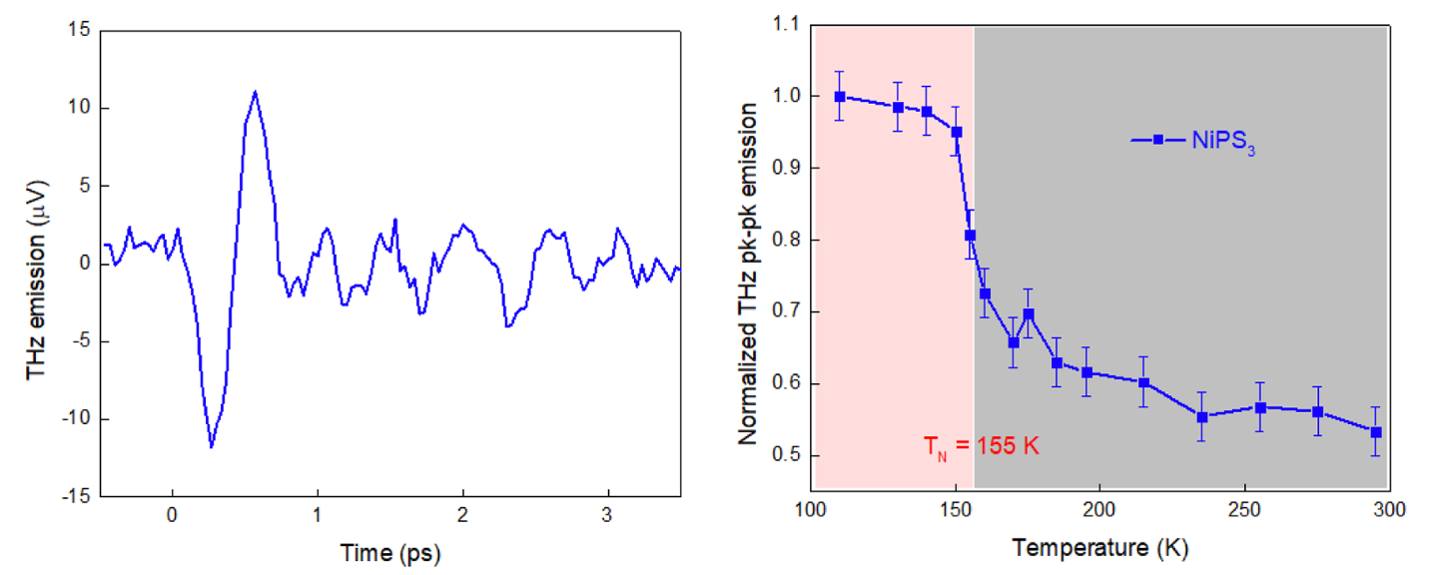
\includegraphics[width=0.7\linewidth]{figures/NiPS3}
	\caption{
		(left)  Measured THz electric field waveform emitted from \(\mathrm{NiPS_3}\) antiferromagnetic sample under femtosecond \(400~\mathrm{nm}\) excitation.
		(right) Peak THz emission amplitude as a function of temperature, showing strong enhancement at the Neel temperature (\(155~\mathrm{K}\)), showing direct sensitivity to time-dependent magnetization.
	}
	\label{fig:NiPS3}
\end{figure}

Several ongoing experimental and theory collaborations from this team are in progress.

\paragraph{Spin dynamics in layered antiferromagnets}\label{sec:2dafm}

In collaboration with {\bf Tan} and {\bf Pemmaraju}, {\bf Lindenberg} has been investigating the ultrafast dynamical response of two-dimensional antiferromagnetic materials.
In antiferromagnets, electron exchange interactions result in antiparallel or non-collinear microscopic spin correlations with negligible macroscopic magnetization.
Given their low-loss, intrinsic THz frequencies, and insensitivity to stray fields, antiferromagnetic spintronics holds great potential in realizing high-speed communications and new types of information storage technologies. 
Atomically-thin van der Waals crystals like \(\mathrm{FePS_3}\), \(\mathrm{NiPS_3}\) and \(\mathrm{MnPS_3}\) represent a new type of antiferromagnetic materials class with strong 2D quantum confinement and the ability to tune this functionality at high speed and with low energy cost, taking advantage of the weak interlayer van der Waals bond.
In initial work, we carried out time-domain THz emission spectroscopy probing the ultrafast dynamics of the magnetization in exfoliated flakes of \(\mathrm{NiPS_3}\).
% In these experiments an ultrafast optical pump pulse excites above band gap at \(400~\mathrm{nm}\) to create free carriers which then couple to the intrinsic magnetization of the material.
By detecting the emitted THz fields from the sample, we probe the time-dependent free (associated with the flow of electrons) and bound (associated with the time-dependent magnetization) currents.
% Following directly from Maxwell’s equations one finds: 

% \begin{equation}
% \mathbf{E}_\text{THz} \propto \frac{\partial\mathbf{J}}{\partial t} + \frac{\partial}{\partial t} (\nabla \times \mathbf{M})
% \end{equation}
% where \(\mathbf{J}\) is the free current and \(\mathbf{M}\) is magnetization. 
Figure~\ref{fig:NiPS3} shows the experimentally measured THz waveform and the peak-to-peak emission amplitude as a function of temperature, showing an enhancement at the Neel temperature.
% This demonstrates the sensitivity of the measurement to the intrinsic antiferromagnetic dynamics.
% Further, by measuring the polarization state of the emitted THz fields one can extract information about the crystallographic directions of the associated currents.
There are two contributions to the measured fields involving a current normal to the sample surface associated with the separation of electrons and holes at the surface superposed on a bound current likely associated with an induced rotation of the initially in-plane antiferromagnetic magnetization state.
Further spectral analysis of the emitted fields may allow us to extract information about particular magnons associated with the light-induced response.
This work opens new possibilities for controlling the properties of antiferromagnetic materials on ultrafast time-scales. 
Ongoing work also involves experiments at the SLAC Ultrafast Electron Diffraction facility where we will investigate the correlated structural dynamics under similar photoexcitation conditions.

In conjunction with this experimental work, {\bf Tan} and {\bf Pemmaraju} are investigating a number of theoretical approaches to this problem.
First, static, first-principles DFT are used to solve for the electronic structure, phononic properties, and electron-phonon interactions of the \(\mathrm{NiPS_3}\) materials system. 
Second, we will use the RT-TDDFT approach to directly simulate density and spin fluctuations in time using the \textsc{INQ} code.
The evolution of the calculated diffraction intensities of the spin, charge, and orbital patterns will provide dynamics of the order parameters to assist the experimental time-resolved diffraction study.
We will examine trajectories to understand the structural and electronic mechanisms behind the evolution of spin order peaks, and their associated time scales. 
Finally, the RT-TDDFT simulations will provide data for parameterization of a model for long-wavelength magnon simulations developed by \textbf{PD Rajpurohit} and \textbf{PI Tan}. 
% This semi-classical approach involves the construction of an effective spin Hamiltonian consisting of Zeeman, exchange and anisotropic magnetic interactions, with parameters extracted from the \textsc{inq} code. 
% This Hamiltonian will be solved for large magnetic supercell to produce the spin-wave dispersions. 
% Development of this model will be accelerated by the team's recent experience with similar models for 2D TMDCs and manganites~\cite{Siddiqui2020, Rajpurohit2020}. 
% As a by-product of this work, the \textsc{inq} code will contain an interface that will facilitate user extraction of parameters for model simulations.

\paragraph{Demagnetization in optically excited perovskite nickelates}

The perovskite nickelates \(\mathrm{RNiO_3}\) are host to a number of unique structural, electronic, and magnetic transitions~\cite{Giovannetti2009,Hampel2017,Beyerlein2018}.
The melting of the low-temperature antiferromagentic order in photoexcited nickelates~\cite{Caviglia2013} is suggested to be directly linked to the melting of charge order, but the details and control of this coupling are not well understood. 
The metal-insulator transition involves structural changes that split \(\mathrm{Ni^{3+}}\) ions to two inequivalent sites, which surprisingly do not involve any Jahn-Teller distortion, unlike typical charge-transfer transitions in other oxide perovskites. 
We will address these unresolved questions using a combination of real-time TDDFT simulation ({\bf Tan}) and time domain THz emission spectroscopy together with Ultrafast Electron Diffraction ({\bf Lindenberg}). 
Similar to the approach to be taken in Section~\ref{sec:2dafm}, this combination of experimental techniques will measure antiferromagnetic dynamics together with correlated structural changes. 
Simulation efforts will target the process of charge order melting due to the instantaneous redistribution of charge carriers during photoexcitation process, and the creation of metastable spiral spin structures over \(0.5~\mathrm{ps}\). 
\textsc{inq} scaling will let us extend these calculations to heterostructures, which are of interest due to possible superconductivity in these structures. These simulations will investigate exchange bias effects at the \(\mathrm{RMnO_3}/\mathrm{RNiO_3}\) interface, the modulation of orbital occupation due to strain and interface effects, and energy transfer across the interface during and after photoexcitation.

\paragraph{Non-linear non-equilibrium response in topological materials}

Non-linear optical phenomena arise when light at sufficiently high intensities interacts with matter.
Nonlinear response underlies technologically important physical effects including shift-currents, harmonic generation, and frequency upconversion in photovoltaic and optoelectronics applications, among others.
Recent insights that non-linear responses are intimately tied to the fundamental topological properties of the quantum materials has increased interest in controlling the excited states of these systems with ultrafast pump-probe and nonlinear multidimensional spectroscopies.

The computational studies we propose are inspired by recent joint experiment-theory results reported by PIs {\bf Lindenberg} and {\bf Pemmaraju} on ultrafast non-linear responses in the Weyl semimetal \(\mathrm{WTe_2}\)~\cite{Xiao_2020}. 
Our studies showed that terahertz frequency light pulses induce large amplitude interlayer shear strains in \(\mathrm{WTe_2}\), modulating its symmetry and potentially its topological phase. 
The THz induced shear strains in \(\mathrm{WTe_2}\) were also found to be associated with a large transient modulation of the second harmonic generation (SHG) response whereby in the THz-driven sample, the SHG response is dramatically reduced compared to non-centrosymmetic bulk \(\mathrm{WTe_2}\). 
However, since the low order non-linear response in materials is fundamentally connected with topological quantities such as the Berry connection and Berry curvature, the question remains as to whether the observed transient reduction in SHG is a signature of a topological phase transition involving the annihilation of Weyl nodes in the Bloch band structure or that of a structural transition to a centrosymmetric geometry.

%We will investigate the electronic \emph{vs.} structural origins of recently observed large transient changes in the second harmonic response of the Weyl semimetal \(\mathrm{WTe_2}\) in response to terahertz-driven lattice modulations.
We will study the relationship between symmetry, topology, and SHG response in \(\mathrm{WTe_2}\) using both frequency and time-domain approaches. Simulations of SHG response in \textsc{inq} will go beyond the BO approximation to model intrinsic non-equilibrium states involving transient field-driven modulations of the electrons and holes near the Weyl band crossing points.
Utilizing the Ehrenfest dynamics capability of the \textsc{inq} code, we plan to investigate the role of transient in-plane currents in driving the observed \(0.24~\mathrm{THz}\) shear-shear responses in \(\mathrm{WTe_2}\), and the role of electron doping in tuning these responses. 
Such studies will contribute significantly to a detailed material specific understanding of ultrafast non-linear response in topological materials within the TMDC family and beyond.

\clearpage

